\chapter{Ergebnisse}\label{chap:Ergebnisse}
Die Vorauslegungwurde mit folgenden Werten durchgeführt:\\
- Isotherm auf: \SI{38}{\celsius}\\
- Avionik Abwärme: \SI{40}{W}\\
- \SI{1}{m} Kontourlänge\\
- Radiator Emissionsgrad: \SI{0,91}{} (AZ-93)\\
- Radiator Absorptionsgrad: \SI{0,15}{} (AZ-93)\\
- Icosane PCM\\
- Trajektoriensimulation\\
- \SI{1}{\frac{kW}{m^2}} mit 50\% dutycycle durch Rotation der Rakete\\
Zu beachten ist, dass die Radiatorleistung konstant bleibt, da das System als isotherm mit einer
infinitesimalen Temperaturerhöhung über den Schmelzpunkt hinweg angenommen wird.
\section{PCM-Radiator-Hybrid}\label{sec:pcmRadiatorHybridErgebnisse}
Als nächstes sieht man Graphen
\begin{figure}[H]
  \centering
  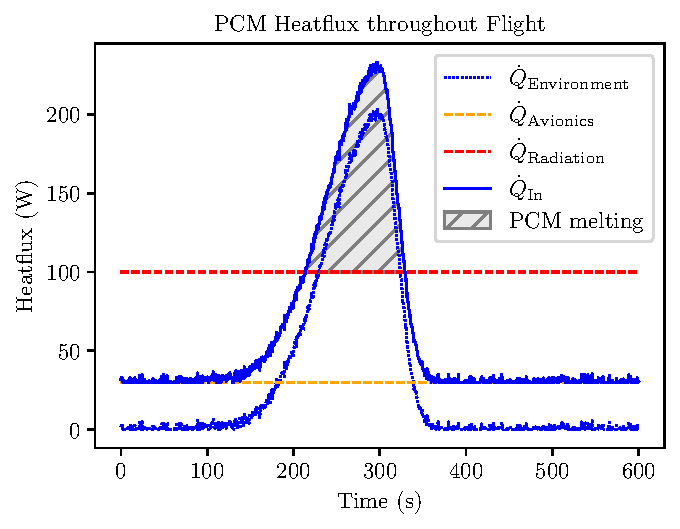
\includegraphics[width=\linewidth]{../../Code/pcm_radiator_hybrid_heatflux_during_flight.pdf}\label{fig:pcm_waermestrom_flugsimulation}
  \caption{PCM Wärmestrom während Flug}
  \includegraphics[width=\linewidth]{../../Code/re_pr_during_flight.pdf}\label{fig:re_pr_flugsimulation}
  \caption{Reynolds- und Prandtlzahl während kritischer Phase im Flug}
\end{figure}